\documentclass[../main.tex]{subfiles}
%\usepackage{algorithm}
%\usepackage{algorithmic}
\everymath{\displaystyle}
\def\arraystretch{2.0}
\begin{document}
\setlength{\delimitershortfall}{0pt}
\section{Optimization}\label{sec:optimization}


As mentioned in REF, the overall motivation for this thesis is optimization. A typicall optimization process, not restricted to fluid problems, is depicted in Figure~\ref{fig:optimization_blockdiagram}.
\begin{figure}[h!]
	\begin{center}
	%/home/lukas/Desktop/project/independence/project/thesis/fig/tikz/build/optimization_blockdiagram.pdf
        \includegraphics{\mainpath/fig/tikz/build/optimization_blockdiagram.pdf}
        \caption[Optimization block-diagram]{Flow chart of an optimization process in the context of flow simulations. If regards the flow-computation block as a black-box to compute gradients of an objective function and the shape-modification block more general as parameter modification, this optimization routine is applicable to all kinds of problems. In our case, we begin with an initial geometry created by a standard mesh-generation software. We also parametrize the initial mesh in terms of design elements in this first step. This is done via SDesign in this thesis. All further modifications to the geometry are obtained via the design element concept. The mesh-movement, steady-state siumulations and \acf{SA} are then performed in AERO-F. For the optimizer itself, python has been chosen in this thesis, more specifically the TODO module. The codes communicate via result-files. These files are used to monitor and investigate the optimization process.}
		\label{fig:optimization_blockdiagram}
    \end{center}
\end{figure}

%\subsection{Basics}\label{sec:basics}

A generic, aeroelastic optimization problem can be written as
\begin{align}
\optcrit(\absvars,\structdisp,\fstate)
&\begin{cases}
&\underset{\absvars}{\text{min }}\costfunc(\absvars) \\%TODO subscribt s
&\eqctr(\absvar)=\vec{0},~~~\eqctr \in \mathbb{R}^{\numeqctr} \\
&\neqctr(\absvar)>\vec{0},~~~\neqctr \in \mathbb{R}^{\numneqctr} \\
\end{cases} \label{eq:generic_optimization_problem_1}\\
&\absvars = \{ \absvars \in \mathbb{R}^{n_{\absvars}} | \absvars_L \leq \absvars \leq \absvars_U \}\label{eq:generic_optimization_problem_2}
\end{align}
Here,  $\costfunc$ is an arbitrary cost function that should be minimized. Note that a maximization problem can easily be obtained by multiplying the cost function by a factor of $-1$. In aerodynamics, a typical example for a cost function would be the \ac{LDR} ratio of an airfoil. The cost-function is described in terms of so-called \textit{abstract variables}. These can have some physical interpretation, but don't necessarily have to(see Section~\ref{sec:design_model}). Since typically, these optimization problems have no finite solution on an unbounded domain, some restrictions/conditions are introduced. In the airfoil example, we would probably specify a minimum lift that is required to support the configuration. Also a maximum stress for the structure will likely have to be specified. These are classical examples of non-equality constraints, denoted by $\neqctr(\absvars)$ in the above formulation. Constraints can also be formulated in an equality sense, for instance geometrical restrictions due to the turbine suspensions.\\
Furthermore, the abstract optimization variables $\absvars$ themselves are typically restricted by lower($\absvars_L$) and upper($\absvars_U$) bounds.\\
The combinations of objective function~$\costfunc$ and constraints $\eqctr$ and $\neqctr$ is typically denoted as optimization criteria $\optcrit$.
\begin{align}\label{eq:optimization_criteria}
&\optcrit=\optcrit(\absvars,\structdisp,\fstate) \nonumber \\
&\structdisp=\structdisp(\absvars),~~~\fstate=\fstate(\absvars)
\end{align}
This thesis follows the \expression{nested analysis and design approach}, meaning that we assume that $\structdisp$ and $\fstate$ always satisfy the aeroelastic state equations. This means that the state equations are not included in the set of constraints, but the structural displacements $\structdisp$ and the fluid state variables $\fstate$ are determined in each iteration.

As \cite{Maute2001} write, the aeroelastic optimization problem can typically be solved by combining three different numerical approaches:
\begin{itemize}
\item Optimization Model
\item Design Model
\item Analysis Model
\end{itemize}

The optimization model describes the solution of the generic optimization problem\eqref{eq:generic_optimization_problem_1}-\eqref{eq:generic_optimization_problem_2}. For this thesis, a \ac{SQP} has been chosen~\cite{Bonnans2006}.\\
The design model links abstract optimization variables~$\absvars$ to actual shapes, structures, geometries or aerodynamics design parameters. For this purpose SDESIGN, a programm specifically written for \ac{SA} purpose in the \ac{FRG}, has been used during this thesis. Its basic concepts an ideas are described in \cite{Maute2003}.\\
Finally, the analysis model provides concepts of evaluation the optimization criteria. Typically, the optimization criteria depend on $\structdisp$ and $\fstate$ which is why a coupled system of equations has to be solved in every design optimization process. The Sensitivity Analysis (SA) is also part of this model. Aeroelastic analysis and Sensitivity analysis are discussed in Section~\ref{sec:aeroelastic_sa}.

\subsection{Optimization Model}\label{sec:optimization_model}
Optimization problems are typically solved by gradient-based methods. The methods are divided into
\begin{itemize}
\item Primal
\item Dual
\item Penalty-barrier   and
\item Lagrange approaches
\end{itemize}
This thesis focuses on Lagrange approaches. For a thorough analysis and comparison of the different approaches, the interested reader is referred to~\cite{Schittkowski1994}.\\
The Lagrangian approach formulates the optimization problem\eqref{eq:generic_optimization_problem_1}\eqref{eq:generic_optimization_problem_2} as an extreme value problem of the Lagrangian:
\begin{align}\label{eq:lagrangian_of_optimization}
\Lagfunc(\absvars,\lagmultseq,\lagmultsneq)=\costfunc(\absvars))=\T{\lagmultseq} \eqctr(\absvars) + \T{\lagmultsneq}\neqctr(\absvars) \\
\end{align}
Here, $\lagmultseq$ denote the Lagrange multipliers for the equality constraints and $\lagmultsneq$ the Lagrange multipliers for the non-equality constraints.
In fact, one can easily see that the original optimization problem can be obtained as saddle point of the Lagrangian:
\begin{align}\label{eq:saddlepoint_optimization}
\pdfrac{\Lagfunc}{\absvars}&=\pdfrac{\costfunc}{\absvars}=\T{\lagmultseq}\pdfrac{\eqctr}{\absvars}+\T{\lagmultsneq}\pdfrac{\neqctr}{\absvars} \\
\pdfrac{\Lagfunc}{\lagmultseq}&=\eqctr=\vec{0} \\
\pdfrac{\Lagfunc}{\lagmultsneq}&=\T{\lagmultsneq}\neqctr=\vec{0}
\end{align}
The \ac{SQP} method, mention before uses a Newton-Rhapsodon algorithm to solve the above system.



\def\incrabsvars{\Delta \absvars}
\def\incrlagmultsneq{\Delta \lagmultsneq}
\def\incrlagmultseq{\Delta \lagmultseq}

\def\PPLagfuncBYabsvars{\ppdfrac{\Lagfunc}{\absvars}}
\def\PLagfuncBYabsvars{\pdfrac{\Lagfunc}{\absvars}}
\def\PneqctrBYabsvars{\pdfrac{\neqctr}{\absvar}}
\def\PeqctrBYabsvars{\pdfrac{\eqctr}{\absvar}}

\begin{align}\label{eq:saddlepoint_newtonform}
\begin{bmatrix}
\it{\PPLagfuncBYabsvars}                & \it{\PneqctrBYabsvars} & \it{\PeqctrBYabsvars} \\
\it{\lagmultsneq}\it{\PneqctrBYabsvars} & \it{\eqctr}            & \vec{0}               \\
\it{\PeqctrBYabsvars}                   & \vec{0}                & \vec{0}
\end{bmatrix}
	\begin{bmatrix}
	\incrabsvars \\
	\incrlagmultsneq \\
	\incrlagmultseq
	\end{bmatrix}\
	=
    -\begin{bmatrix}
		\it{\PLagfuncBYabsvars} \\
		\T{\it{\lagmultsneq}} \it{\neqctr} \\
		\it{\eqctr}
		\end{bmatrix}
\end{align}
Here $\it{(\cdot)}$ denotes the iteration index of the optimization loop.\\
~\\
The linear Equations~\eqref{eq:saddlepoint_newtonform} can also be formulated as an equivalent quadratic minimization problem:



\begin{align}
\underset{\absvars}{\text{min }}( \frac{1}{2} \T{\incrabsvars} \it{\PPLagfuncBYabsvars} \incrabsvars + \frac{\partial \it{\costfunc}}{\partial \absvars} ) \label{eq:quadratic_minimization_problem_1}\\
\it{\PneqctrBYabsvars} \incrabsvars+\it{\neqctr} \geq \vec{0} \label{eq:quadratic_minimization_problem_2}\\
\it{\PeqctrBYabsvars} \incrabsvars+\it{\eqctr} = \vec{0} \label{eq:quadratic_minimization_problem_3}
\end{align}
\\
In the above formulation, the evaluation of the second derivative of the Lagrangian(Hessian of $\Lagfunc$) is the numerically most expensive part. Usually it is preferred to approximate it by a first-order information, for example by the \ac{DFP} or by the \ac{BFGS} method. However, this simplification introduces an error that one should be aware of. Some correction methods have been proposed trying to minimize the error. In this thesis we adapt the one proposed by~\cite{Maute2001}:
\begin{align}\label{eq:correction_step}
\begin{bmatrix}
\absvars^{(k+1)} \\
\lagmultseq^{(k+1)} \\
\lagmultsneq^{(k+1)}
\end{bmatrix} =
  \begin{bmatrix}
  \it{\absvars} \\
  \it{\lagmultseq} \\
  \it{\lagmultsneq} \\
  \end{bmatrix} +
    \it{\alpha}
    \begin{bmatrix}
    \it{\incrabsvars} \\
    \it{\incrlagmultseq} \\
    \it{\incrlagmultsneq} \\
    \end{bmatrix}
\end{align}
The appropriate step size $\it{\alpha}$ is determined by a line search. AS~\cite{Maute2001} write, due to this insufficiencies, the Lagrangian can not be used to measure an improvement. Instead, a merit function is introduced that is minimized by the line-search. A local minimum is reached by following a sequence of decreasing merit function values. Convergence of the process can be measured via the $\mathcal{L}_2$-norm of the residual of the Kuhn-Tucker conditions\eqref{eq:saddlepoint_optimization}.\\
By construction, the constraints are satisfied only when the optimum point is reached.



%
\subsection{Design Model}\label{sec:design_model}
The design model represent the essential link between the described optimization model and the analysis model. Generally speaking, it relates physical design parameters to abstract ones.
\begin{align}
\physvars=\physvars(\absvars),~~~\physvars \in \mathbb{R}^{n_{\physvars}} \label{eq:physvarsTOabsvars}
\end{align}
Here, $n_{\physvars}$ denotes the number of physical design parameters.
To define a relation between the abstract optimization variables and the motion of the nodes, the following design model is introduced:
\begin{align}
\mms=\mms(\absvars)
\end{align}

As~\cite{Maute2001} explain, it is unpractical to identify an abstract variable directly with an increment of the coordinate of a grid point. Instead, two approaches, namely geometrical and mechanical can be adopted for constructing the generic design model.
\paragraph{Mechanical approach}
In the mechanical approach, the shape variation is identified with a superposition of fictitious structural deformations $\fic{\structdisp}_{j}$ due to fictitious loads $\mu \fic{\vec{P}}_{j}$ and fictions support conditions
\begin{align}
\mms=\sum_j \fic{\structdisp}_j = \sum_j \inv{\fic{\stiffmat}_j} \mu_j \fic{\vec{P}}_{j} \label{eq:mechanical_approach}
\end{align}
where $\fic{\stiffmat}_j$ is a fictitious pseudo structure stiffness matrix representing the fluid domain compatible to the current fictions support conditions.

\paragraph{Geometrical approach}
The geometrical approach describes the geometry of the structure or the fluid boundary the design element concept. Here, the shape of a body $\tensor{X}$ is approximated by so-called design elements as follows:
\begin{align}
\tensor{X}=\sum_{j} \phi_{j}(\xi) \hat{\tensor{X}}_j \label{eq:geometrical_approach}
\end{align}
Here, $\phi_{j}(\xi)$ is a shape function, $\hat{\tensor{X}}_j$ is the vector of control nodes and $\xi$ represents the reference coordinate. In the design element concept, the variation of the control nodes of the design element is used to vary the shape of the body. The variation of the control nodes position denoted as "mesh-motion" is given as $\mms=\Delta \hat{\tensor{X}} $
\begin{align}
\mms = \sum_j \phi_{j}(\xi) \hat{\mms}_j \label{eq:mms}
\end{align}

Just as in Finite Elements, where the shape-functions can not only be used to describe the solution field, but also the body's geometry and material parameters, the design element concept can be applied to prescribe parameter distributions and their variations in the optimization process. A simple sketch of the concept is provided in Figure~\ref{fig:sketch_geometrical_approach}
\\
Both approaches have pros and cons, that are quickly discussed in \cite{Maute2003}, this thesis utilizes the geometrical approach solemnly.

\begin{figure}[h!]
	\begin{center}
        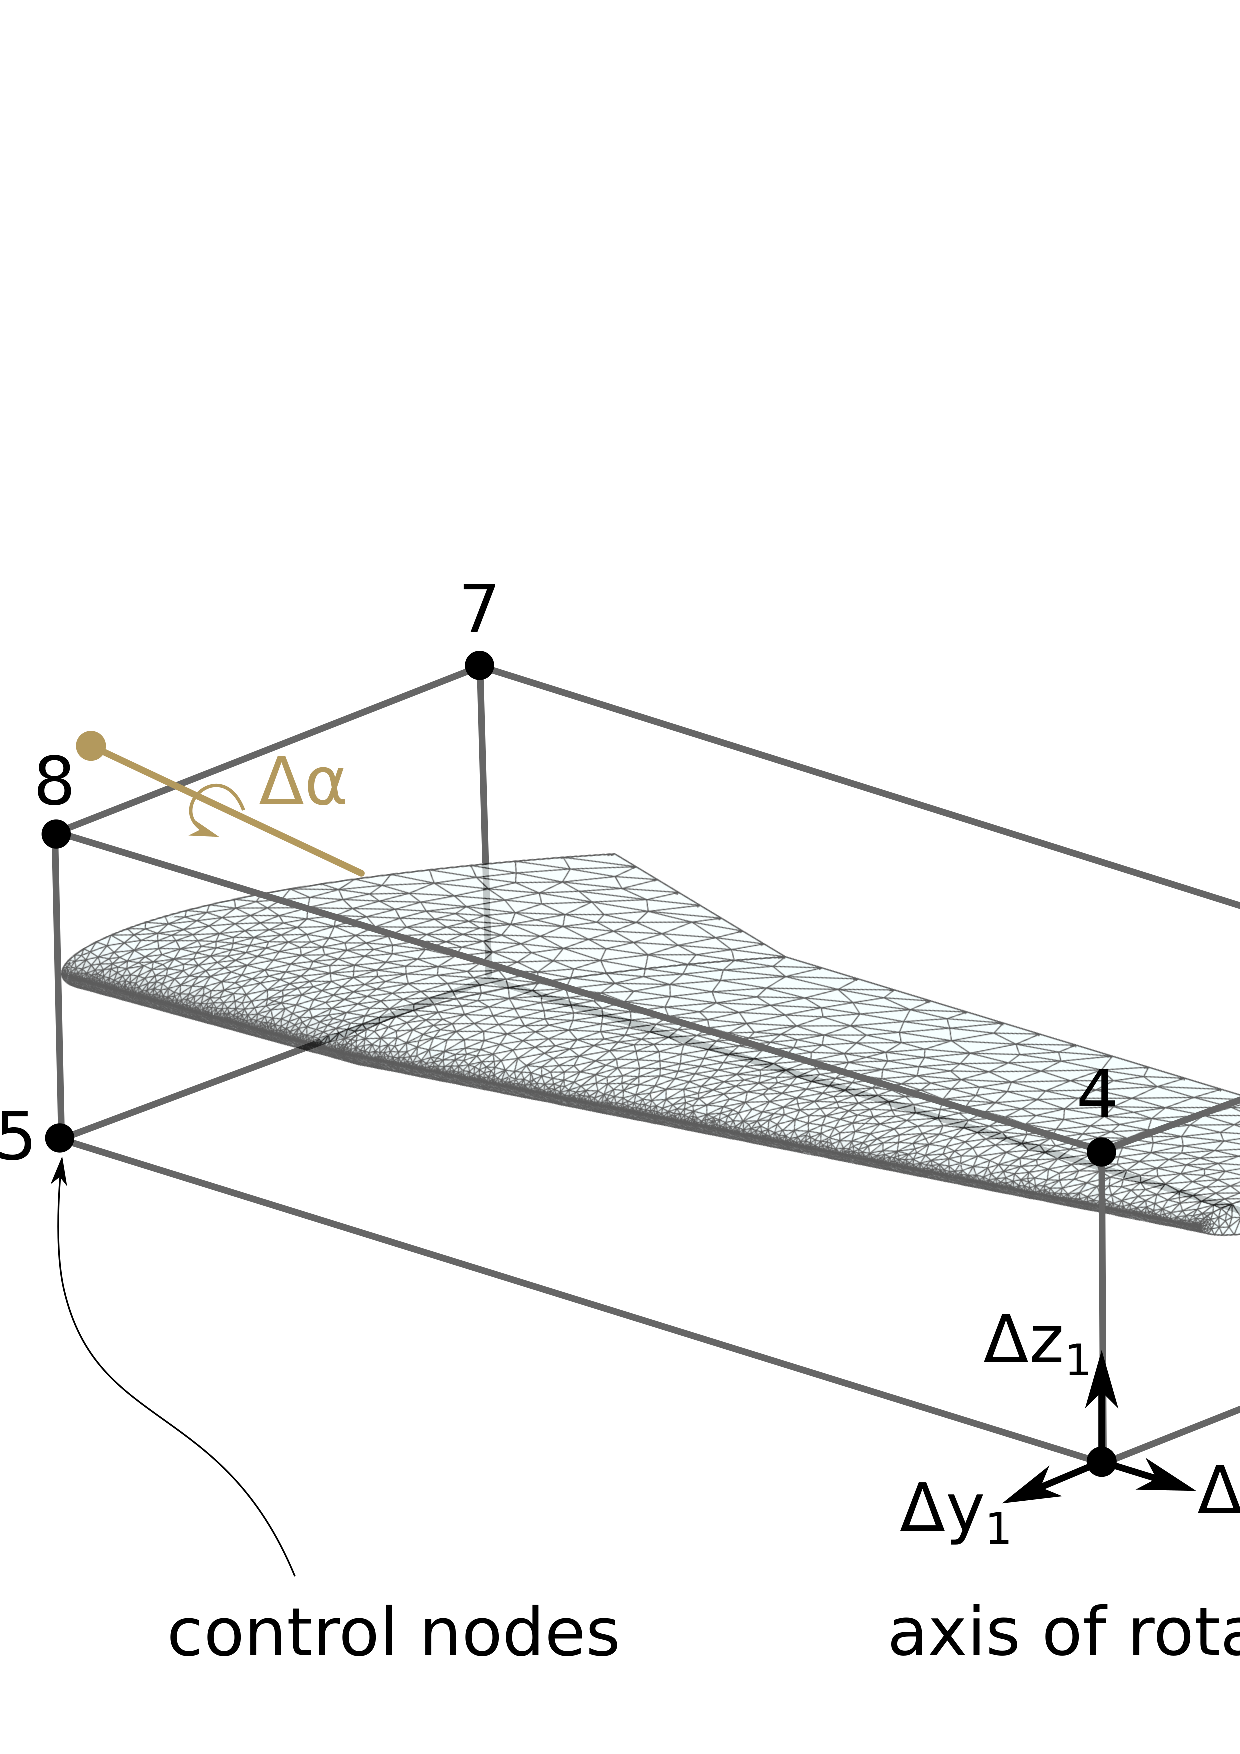
\includegraphics[width=1.0\textwidth]{\mainpath/fig/pdf/sdesign.pdf}
        \caption[Design-model: geometrical approach]{Geometrical approach for the design model as explained in Section~\ref{sec:design_model}. A NACA type airfoil is considered here as an example. The airfoil is embedded in a bounding box defined by eight so-called control nodes. The position of these control nodes can be varied, which alternates the shape of the airfoil according to some interpolation functions defined on the nodes. The 24 displacement unknowns are denoted as "abstract shape parameters". Abstract shape variables can be arbitrarily defined. As an example, a rotation axis is defined through the wing.}
		\label{fig:sketch_geometrical_approach}
    \end{center}
\end{figure}

\begin{figure}[h!]
	\begin{center}
        \includegraphics{\mainpath/fig/tikz/build/sdesign_visualization.pdf}
        \caption[Design element visualization]{Visualization of the design element concept, exemplarily shown on a NACA0012 airfoil. For simplicity, a single design element(cubic in the horizontal direction and linear in the vertical direction) is used. Both the initial configuration(dashed lines) and the deformed configuration(full lines) are plotted. Although only eight design element nodes are provided, the function space of the design element allows for a great variation of the airfoil shape. Also, the size of the parameter space is now independent of the airfoil mesh size. From this perspective, the design element concept can be regarded as an model reduction for the shape variation.}
		\label{designelement_concept_2D}
    \end{center}
\end{figure}

%TODO talk about SDESIGN
\subsection{Analysis Model}\label{sec:analysis_model}
In the analysis model, the optimization criteria $\optcrit$ are determined for a given set of obtimization variables $\absvar$. Since the optimization algorithm choses in this thesis is based on gradients, the gradients of the optimization criteria with respect to the abstract variables are determined in this step. A main focus on this thesis has been the appropriate evaluation of these derivatives, we therfore denote the subsequent chapter~\ref{sec:SA} to the issue.

\end{document}
